\documentclass [12pt, a4paper, english, brazil, oneside, chapter=TITLE, section=TITLE]{abntex2}
% Para impressão use doubleside
% ---
% Arquivo com  a formatação é lido aqui. Não deve ser modificado
% ---
\usepackage[utf8]{inputenc}
\usepackage[T1]{fontenc}
\usepackage{amsmath}
\usepackage{amssymb,amsfonts,textcomp}
\usepackage{color}
\usepackage{array}
\usepackage{supertabular}
\usepackage{listings}         % Para as linguagens de programação
\usepackage{lastpage}		  % Usado pela Ficha catalográfica
\usepackage{indentfirst}	  % Indenta o primeiro parágrafo de cada seção.
\usepackage{hhline}
\usepackage{hyperref}
% Informações do PDF
\hypersetup{ colorlinks=false, linkcolor=blue, citecolor=blue, filecolor=blue, urlcolor=blue, pdftitle=DEPARTAMENTO DE CIÊNCIA DA COMPUTAÇÃO - UFRJ, pdfauthor=, pdfsubject=, pdfkeywords=}

\usepackage[pdftex]{graphicx}
\graphicspath{ {./figuras/} }
% ---
% Pacotes glossaries
% ---
\usepackage[subentrycounter,seeautonumberlist,nonumberlist=true]{glossaries}
% para usar o xindy ao invés do makeindex:
%\usepackage[xindy={language=portuguese},subentrycounter,seeautonumberlist,nonumberlist=true]{glossaries}
% ---
% Citações de referências no formato alfabético e negrito
\usepackage[alf, abnt-emphasize=bf]{abntex2cite}
% Margens definidas em 25 mm para uso como documento em PDF
% Para imprimir use as seguintes margens:
% \usepackage[left=30mm, top=30mm, right=20 mm, bottom=20mm] {geometry}

\usepackage[margin=25 mm]{geometry}

%%%%%%%%%%%%%%%%%%%%%%%%%%%%%%%%%%%%%%%%%%%%%%%%%%%%%%%%%%%%%
% Definições de Macros utilizadas no TCC
%%%%%%%%%%%%%%%%%%%%%%%%%%%%%%%%%%%%%%%%%%%%%%%%%%%%%%%%%%%%%
\instituicao{UNIVERSIDADE FEDERAL DO RIO DE JANEIRO
\par
INSTITUTO DE MATEMÁTICA
\par
CURSO DE BACHARELADO EM CIÊNCIA DA COMPUTAÇÃO}
\title{MODELO DE MONOGRAFIA DE TRABALHO DE CONCLUSÃO DE CURSO\\ Modelo em Latex}
\author{Gabriel P. Silva}
\autor{Ana Lisa M. Dias \\ Oscar A. Melo}
\orientador{Prof. João José da Silva}
\coorientador{Profa. Maria da Penha}
\local{RIO DE JANEIRO}
\data{2018}
\preambulo{Trabalho de conclusão de curso de graduação apresentado ao Departamento de Ciência da Computação da Universidade Federal do Rio de Janeiro como parte dos requisitos para obtenção do grau de Bacharel em Ciência da Computação.}

\usepackage{tocloft}

\usepackage{pdfpages}

%%%%%%%%%%%%%%%%%%%%%%%%%%%%%%%%%%%%%%%%%%%%%%%%%%%%%%%%%%%
% Corrige a fonte dos capítulos, seções, resumos, etc.
%%%%%%%%%%%%%%%%%%%%%%%%%%%%%%%%%%%%%%%%%%%%%%%%%%%%%%%%%%%
\renewcommand{\ABNTEXchapterfont}{\bfseries \rmfamily}
\renewcommand{\ABNTEXchapterfontsize}{\normalsize}

\renewcommand{\ABNTEXsectionfont}{\mdseries}
\renewcommand{\ABNTEXsectionfontsize}{\normalsize}

\renewcommand{\ABNTEXsubsectionfont}{\bfseries}
\renewcommand{\ABNTEXsubsectionfontsize}{\normalsize}

\renewcommand{\lstlistingname}{Código}
\renewcommand{\lstlistlistingname}{Lista de \lstlistingname s}

%%%%%%%%%%%%%%%%%%%%%%%%%%%%%%%%%%%%%%%%%%%%%%%%%%%%%%%%%%%
% Criação de quadros com numeração
%%%%%%%%%%%%%%%%%%%%%%%%%%%%%%%%%%%%%%%%%%%%%%%%%%%%%%%%%%%
\newcommand{\quadroname}{Quadro}
\newcommand{\listofquadrosname}{Lista de quadros}

\newfloat[chapter]{quadro}{loq}{\quadroname}
\newlistof{listofquadros}{loq}{\listofquadrosname}
\newlistentry{quadro}{loq}{0}

% configurações para atender às regras da ABNT
\setfloatadjustment{quadro}{\centering}
\counterwithout{quadro}{chapter}
\renewcommand{\cftquadroname}{\quadroname\space}
\renewcommand*{\cftquadroaftersnum}{\hfill--\hfill}

% Configuração de posicionamento padrão:
\setfloatlocations{quadro}{hbtp}

% Para ajudar nas tabelas e quadros
\makeatletter
\newcommand\arraybslash{\let\\\@arraycr}
\makeatother

%%%%%%%%%%%%%%%%%%%%%%%%%%%%%%%%%%%%%%%%%%%%%%%%%%%%%%%
% Redefine a macro para imprimir a capa
%%%%%%%%%%%%%%%%%%%%%%%%%%%%%%%%%%%%%%%%%%%%%%%%%%%%%%%
\renewcommand{\imprimircapa}{%
\begin{capa}%
\center
\imprimirinstituicao
\par
\vspace*{1cm}
\MakeUppercase{\imprimirautor}
\vfill
\begin{center}
\imprimirtitulo
\end{center}
\vfill
\imprimirlocal
\par
\imprimirdata
\vspace*{1cm}
\end{capa}
}
%%%%%%%%%%%%%%%%%%%%%%%%%%%%%%%%%%%%%%%%%%%%%%%%%%%%%%%
% Redefine a macro para imprimir a folho de rosto
%%%%%%%%%%%%%%%%%%%%%%%%%%%%%%%%%%%%%%%%%%%%%%%%%%%%%%%
\renewcommand{\imprimirfolhaderosto}{%
\begin{capa}%
\center
\par
\vspace*{1cm}
\MakeUppercase{\imprimirautor}
\vfill
\begin{center}
\imprimirtitulo
\end{center}
\vfill
\hspace*{\fill}\parbox[b]{.5\textwidth}{%
        \linespread{1}\selectfont
\imprimirpreambulo
}
\vfill
\flushright
Orientador: \imprimirorientador\\

Co-orientador: \imprimircoorientador\\
\vfill
\begin{center}
\large\imprimirlocal
\par
\large\imprimirdata
\vspace*{1cm}
\end{center}
\end{capa}
}

%%%%%%%%%%%%%%%%%%%%%%%%%%%%%%%%%%%%%%%%%%%%%%%%%%%%
% Definição das Linguagens de Programação
%%%%%%%%%%%%%%%%%%%%%%%%%%%%%%%%%%%%%%%%%%%%%%%%%%%%
\definecolor{dkgreen}{rgb}{0,0.6,0}
\definecolor{gray}{rgb}{0.5,0.5,0.5}
\definecolor{purple}{rgb}{0.8,0,0.3}
\definecolor{orange}{rgb}{1,0.4,0}
\definecolor{lightlightgray}{rgb}{.95,.95,.95}
\definecolor{lightgray}{rgb}{.9,.9,.9}
\definecolor{lightgray2}{rgb}{.85,.85,.85}
\definecolor{darkgray}{rgb}{.4,.4,.4}

% Comando para inserir a listagem de código, tem 4 parâmetros
% Linguagem, Caption, Label, Nome do Arquivo
\newcommand{\includecode}[4][C]{\mbox{\lstinputlisting[caption=#2, label=#3, escapechar=, style=custom#1]{#4}}}


%Define características em comum
\lstset{framexleftmargin=5mm,  frame=shadowbox, rulesepcolor=\color{gray}}

% Aqui você pode customizar a linguagem
\lstdefinestyle{customC}{
      language = C,
      breaklines=true,
      basicstyle=\footnotesize\ttfamily,
      keywordstyle=\bfseries\color{blue},
      commentstyle=\itshape\color{purple},
      identifierstyle=\color{black},
      stringstyle=\color{orange},
      showstringspaces=false}

% Aqui você pode customizar a linguagem
\lstdefinestyle{customJava}{
      language = Java,
      breaklines=true,
      basicstyle=\footnotesize\ttfamily,
      keywordstyle=\bfseries\color{blue},
      commentstyle=\itshape\color{purple},
      identifierstyle=\color{black},
      stringstyle=\color{orange},
      showstringspaces=false}

% Aqui você pode customizar a linguagem
\lstdefinestyle{customC++}{
      language = C++,
      breaklines=true,
      basicstyle=\footnotesize\ttfamily,
      keywordstyle=\bfseries\color{blue},
      commentstyle=\itshape\color{purple},
      identifierstyle=\color{black},
      stringstyle=\color{orange},
      showstringspaces=false}

\lstdefinestyle{customJavaScript}{
      language = JavaScript,
      breaklines=true,
      basicstyle=\footnotesize\ttfamily,
      keywordstyle=\bfseries\color{blue},
      commentstyle=\itshape\color{purple},
      identifierstyle=\color{black},
      stringstyle=\color{orange},
      showstringspaces=false}

\lstdefinestyle{customJSON}{
      language = JSON,
      breaklines=true,
      basicstyle=\footnotesize\ttfamily,
      keywordstyle=\bfseries\color{blue},
      commentstyle=\itshape\color{purple},
      identifierstyle=\color{black},
      stringstyle=\color{orange},
      showstringspaces=false}

\lstdefinestyle{customSapiens}{
      language = Sapiens,
      breaklines=true,
      basicstyle=\footnotesize\ttfamily,
      keywordstyle=\bfseries\color{blue},
      commentstyle=\itshape\color{purple},
      identifierstyle=\color{black},
      stringstyle=\color{orange},
      showstringspaces=false}

% Javascript
\lstdefinelanguage{JavaScript}{
    aboveskip=15pt,
    keywords={typeof, new, true, false, catch, function, return, null, catch, switch, var, if, in, while, do, else, case, break},
    keywordstyle=\color{blue}\bfseries,
    ndkeywords={class, export, boolean, throw, implements, import, this},
    ndkeywordstyle=\color{darkgray}\bfseries,
    identifierstyle=\color{black},
    sensitive=false,
    comment=[l]{//},
    morecomment=[s]{/*}{*/},
    commentstyle=\color{purple}\ttfamily,
    stringstyle=\color{red}\ttfamily,
    morestring=[b]',
    morestring=[b]",
    rulecolor=\color{lightgray2},
    breaklines=true,
    basicstyle=\footnotesize\ttfamily,
    frame=single,
    backgroundcolor=\color{lightlightgray}
}
% JSON
\lstdefinelanguage{JSON}{
    aboveskip=15pt,
    string=[s]{"}{"},
    stringstyle=\color{blue},
    comment=[l]{:},
    commentstyle=\color{black},
    rulecolor=\color{lightgray2},
    breaklines=true,
    basicstyle=\footnotesize\ttfamily,
    frame=single,
    backgroundcolor=\color{lightlightgray}
}

% Linguagem de Montagem
\lstdefinelanguage{Sapiens}{
    aboveskip=15pt,
    keywordstyle=\color{blue}\bfseries,
    comment=[l]{;},
    commentstyle=\color{purple},
    rulecolor=\color{lightgray2},
    breaklines=true,
    basicstyle=\footnotesize\ttfamily,
    frame=single,
    backgroundcolor=\color{lightlightgray},
    language=[x86masm]Assembler,
    morekeywords={DB, DS, DW, JN, JSR, LDA, ORG, STA, STS, TRAP}
}

% ---
% GLOSSARIO
% ---
\makeglossaries
% ---
% entradas do glossário
% ---

\newglossaryentry{pai}{
	name={pai},
	plural={pai},
	description={este é uma entrada pai, que possui outras
			subentradas.} }

\newglossaryentry{componente}{
	name={componente},
	plural={componentes},
	parent=pai,
	description={descriação da entrada componente.} }

\newglossaryentry{filho}{
	name={filho},
	plural={filhos},
	parent=pai,
	description={isto é uma entrada filha da entrada de nome
			\gls{pai}. Trata-se de uma entrada irmã da entrada
			\gls{componente}.} }

\newglossaryentry{equilibrio}{
	name={equilíbrio da configuração},
	see=[veja também]{componente},
	description={consistência entre os \glspl{componente}}
}

\newglossaryentry{latex}{
	name={LaTeX},
	description={ferramenta de computador para autoria de
			documentos criada por D. E. Knuth} }

\newglossaryentry{abntex2}{
	name={abnTeX2},
	see=latex,
	description={suíte para LaTeX que atende os requisitos das
			normas da ABNT para elaboração de documentos técnicos e científicos brasileiros} }
% ---
%\item [Palavra] Significado da palavra

%\item [Palavra 2] Significado da palavra 2
% ---
%%%%%%%%%%%%%%%%%%%%%%%%%%%%%%%%%%%%%%%%%%%%%%%%%%%%%%%%%%%%
% I N I C I O  D O  D O C U M E N T O
%%%%%%%%%%%%%%%%%%%%%%%%%%%%%%%%%%%%%%%%%%%%%%%%%%%%%%%%%%%%
\begin{document}
\pretextual

%%%%%%%%%%%%%%%%%%%%%%%%%%%%%%%%%%%%%%%%%%%%%%%%%%%%%%%%%%%%
% C A P A (OBRIGATÓRIO)
%%%%%%%%%%%%%%%%%%%%%%%%%%%%%%%%%%%%%%%%%%%%%%%%%%%%%%%%%%%%

\setcounter{page}{1}
\imprimircapa

%%%%%%%%%%%%%%%%%%%%%%%%%%%%%%%%%%%%%%%%%%%%%%%%%%%%%%%%%%%%
% F O L H A  D E  R O S T O  (OBRIGATÓRIO)
%%%%%%%%%%%%%%%%%%%%%%%%%%%%%%%%%%%%%%%%%%%%%%%%%%%%%%%%%%%%

\imprimirfolhaderosto

%%%%%%%%%%%%%%%%%%%%%%%%%%%%%%%%%%%%%%%%%%%%%%%%%%%%%%%%%%%%
% F I C H A   C A T A L O G R Á F I A  (OBRIGATÓRIO)
%%%%%%%%%%%%%%%%%%%%%%%%%%%%%%%%%%%%%%%%%%%%%%%%%%%%%%%%%%%%
% Ficha catalográfica (obrigatório)
% Para elaborar a ficha catalográfica siga as instruções em
% http://fichacatalografica.sibi.ufrj.br/}
%%%%%%%%%%%%%%%%%%%%%%%%%%%%%%%%%%%%%%%%%%%%%%%%%%%%%%%%%%%%
\vspace*{1cm}
\begin{fichacatalografica}
\begin{figure}[b]
\centering
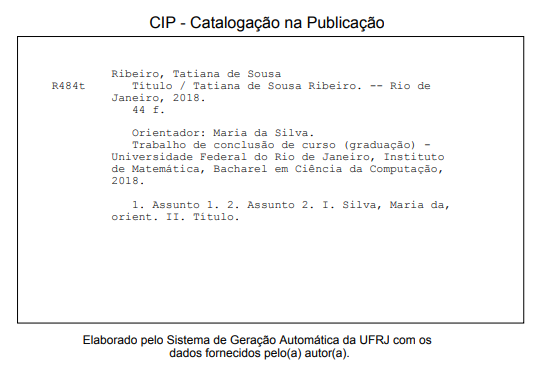
\includegraphics[width=14.217cm,height=9.929cm]{ModeloMonografiaDCCUFRJ-img001.png}
\end{figure}
% Opcionalmente você pode usar
% \includepdf{fig_ficha_catalografica.pdf}
\end{fichacatalografica}

%%%%%%%%%%%%%%%%%%%%%%%%%%%%%%%%%%%%%%%%%%%%%%%%%%%%%%%%%
% F O L H A   D E   A P R O V A Ç Ã O  (OBRIGATÓRIO)
%%%%%%%%%%%%%%%%%%%%%%%%%%%%%%%%%%%%%%%%%%%%%%%%%%%%%%%%%
% Isto é um exemplo folha de aprovação.
% Substitua todo o conteúdo desta página por uma
% imagem da página assinada pela banca com o comando abaixo:
% \includepdf{folhadeaprovacao_final.pdf}
%%%%%%%%%%%%%%%%%%%%%%%%%%%%%%%%%%%%%%%%%%%%%%%%%%%%%%%%%

\begin{folhadeaprovacao}
\vspace*{\fill}
\begin{center}
    {\MakeUppercase{\imprimirautor}} 
    \vspace*{\fill}
    \begin{center}
      \imprimirtitulo \\
    \end{center}
    \vspace*{\fill}
  \end{center}
  \hspace*{\fill}\parbox[b]{.5\textwidth}{%
    \linespread{1}\selectfont
    \imprimirpreambulo
}

\vspace*{\fill}
    \begin{flushleft}
 % Alterar a data ou preencher à mão
   Aprovado em \_\_\_ de \_\_\_\_\_\_\_\_\_\_\_\_\_\_ de \_\_\_\_\_\_\_
  \par
  \vspace*{\fill}

BANCA EXAMINADORA:
\end{flushleft}

  \vspace*{\fill}
   \assinatura{Nome do Professor Orientador \\ Titulação (Instituição)}
   \vspace*{\onelineskip}
   \assinatura{Nome do Professor1 \\ Titulação (Instituição)}
   \vspace*{\onelineskip}
   \assinatura{Nome do Professor2\\ Titulação (Instituição)}
   %\assinatura{Nome do Professor, Titulação (Instituição)}
   %\assinatura{Nome do Professor, Titulação (Instituição)}
\vspace*{\fill}
\end{folhadeaprovacao}


%%%%%%%%%%%%%%%%%%%%%%%%%%%%%%%%%%%%%%%%%%%%%%%%%%%%%%%%%%%
% D E D I C A T O R I A  (OPCIONAL)
%%%%%%%%%%%%%%%%%%%%%%%%%%%%%%%%%%%%%%%%%%%%%%%%%%%%%%%%%%%

\begin{dedicatoria}
	\vspace*{\fill}
	Dedicatória: Texto no qual o autor do trabalho oferece homenagem ou
	dedica o seu trabalho a alguém.
	\vspace*{\fill}
\end{dedicatoria}

%%%%%%%%%%%%%%%%%%%%%%%%%%%%%%%%%%%%%%%%%%%%%%%%%%%%%%%%%%%%
% A G R A D E C I M E N T O S  (OPCIONAL)
%%%%%%%%%%%%%%%%%%%%%%%%%%%%%%%%%%%%%%%%%%%%%%%%%%%%%%%%%%%%

\begin{agradecimentos}
	Os agradecimentos devem ser dirigidos àqueles que contribuíram de
	maneira relevante à elaboração do trabalho,
	restringindo-se ao mínimo necessário, como instituições (CNPq, CAPES,
	UFRJ, empresas ou organizações que fizeram parte
	da pesquisa), ou pessoas (profissionais, pesquisadores, orientadores,
	etc.).

	Os agradecimentos devem ser colocados de forma hierárquica de
	importância e para trabalhos financiados com recursos de
	instituições (CAPES, CNPq, FINEP, FAPERJ, etc.) os agradecimentos são
	obrigatórios a essas instituições.
\end{agradecimentos}

%%%%%%%%%%%%%%%%%%%%%%%%%%%%%%%%%%%%%%%%%%%%%%%%%%%%%%%%%%%%
% E P I G R A F E (OPCIONAL E SEM TÍTULO)
%%%%%%%%%%%%%%%%%%%%%%%%%%%%%%%%%%%%%%%%%%%%%%%%%%%%%%%%%%%%

\begin{epigrafe}
	\vspace*{\fill}
	\begin{flushright}
		Epígrafe: É um item onde o autor apresenta a citação de um texto que seja relacionado com o tema do trabalho, seguido da indicação de autoria do mesmo.\\
		(texto iniciando do meio da página alinhado à direita)\\
		\vspace{\onelineskip}
		\textit{‘‘Few are those who see with their \\
			own eyes and feel with their own hearts."\\}
		\vspace{\onelineskip}
		{\bfseries
			Albert Einstein
			\par}
		(Nome do autor da epígrafe)
	\end{flushright}
\end{epigrafe}


%%%%%%%%%%%%%%%%%%%%%%%%%%%%%%%%%%%%%%%%%%%%%%%%%%%%%%%%%%%%
% R E S U M O    E M    P O R T U G U Ê S  (OBRIGATÓRIO)
%%%%%%%%%%%%%%%%%%%%%%%%%%%%%%%%%%%%%%%%%%%%%%%%%%%%%%%%%%%%

\begin{resumo}
	\begin{SingleSpace}
		Resumo em português. O texto deve ser digitado ou datilografado em um só parágrafo com \textbf{espaçamento simples} e conter de \textbf{150 a 500} palavras. Utilizar a terceira pessoa do singular, os verbos na voz ativa e evitar o uso de símbolos e contrações que não sejam de uso corrente. O resumo deve ressaltar o  objetivo, o método, os resultados e as conclusões do documento. As palavras-chave devem figurar logo abaixo do resumo, antecedidas da expressão \textbf{Palavras-chave:}, separadas entre si por
		ponto e finalizadas também por ponto.
	\end{SingleSpace}
	\vspace{\onelineskip}
	\textbf{Palavras-chave}: latex. abntex. editoração de texto.

\end{resumo}

% Palavras-chave separadas e finalizadas por ponto




%%%%%%%%%%%%%%%%%%%%%%%%%%%%%%%%%%%%%%%%%%%%%%%%%%%%%%%%%%%%
% A B S T R A C T  (MANDATORY)
%%%%%%%%%%%%%%%%%%%%%%%%%%%%%%%%%%%%%%%%%%%%%%%%%%%%%%%%%%%%

\begin{resumo}[Abstract]
\begin{otherlanguage*}{english}
\begin{SingleSpace}
Abstract in english. The text should be typed or typed in a single paragraph with \textbf{single spacing} and contain between 150 and 500 words. Use the third person singular, the verbs in the active voice and avoid the use of symbols and contractions that are not of
current use.
\end{SingleSpace}

%Eventually you can also write it in spanish \textit{(resumen}), french \textit{(résumé)}, italian \textit{(riassunto)} etc.

\vspace{\onelineskip}
   \textbf{Keywords}: latex. abntex. text editoration.
 \end{otherlanguage*}
\end{resumo}




  


%%%%%%%%%%%%%%%%%%%%%%%%%%%%%%%%%%%%%%%%%%%%%%%%%%%%%%%%%%%%
% L I S T A   D E   I L U S T R A Ç Õ E S  (OPCIONAL)
%%%%%%%%%%%%%%%%%%%%%%%%%%%%%%%%%%%%%%%%%%%%%%%%%%%%%%%%%%%%

\pdfbookmark[0]{\listfigurename}{lof}
\listoffigures*
\cleardoublepage

%%%%%%%%%%%%%%%%%%%%%%%%%%%%%%%%%%%%%%%%%%%%%%%%%%%%%%%%%%%%
% L I S T A   D E   C Ó D I G O S (OPCIONAL)
%%%%%%%%%%%%%%%%%%%%%%%%%%%%%%%%%%%%%%%%%%%%%%%%%%%%%%%%%%%%

\pdfbookmark[0]{\lstlistlistingname}{lol}
\begin{KeepFromToc}
\lstlistoflistings
\end{KeepFromToc}
\cleardoublepage

%%%%%%%%%%%%%%%%%%%%%%%%%%%%%%%%%%%%%%%%%%%%%%%%%%%%%%%%%%%%
% L I S T A   D E   T A B E L A S  (OPCIONAL)
%%%%%%%%%%%%%%%%%%%%%%%%%%%%%%%%%%%%%%%%%%%%%%%%%%%%%%%%%%%%

\pdfbookmark[0]{\listtablename}{lot}
\listoftables*
\cleardoublepage

%%%%%%%%%%%%%%%%%%%%%%%%%%%%%%%%%%%%%%%%%%%%%%%%%%%%%%%%%%%%
% L I S T A   D E   Q U A D R O S (OPCIONAL)
%%%%%%%%%%%%%%%%%%%%%%%%%%%%%%%%%%%%%%%%%%%%%%%%%%%%%%%%%%%%

\pdfbookmark[0]{\listofquadrosname}{loq}
\listofquadros*
\cleardoublepage

%%%%%%%%%%%%%%%%%%%%%%%%%%%%%%%%%%%%%%%%%%%%%%%%%%%%%%%%%%%%
% L I S T A   D E  A B R E V I A T U R A S  E   S I G L A S
% (OPCIONAL)
%%%%%%%%%%%%%%%%%%%%%%%%%%%%%%%%%%%%%%%%%%%%%%%%%%%%%%%%%%%%

\begin{siglas}
	\item[Fig.] Area of the $i^{th}$ component
	\item[456] Isto é um número
	\item[123] Isto é outro número
	\item [Bibliot.] Biblioteconomia
	\item [Inform.]  Informática
	\item [ABNT] Associação Brasileira de Normas Técnicas
	\item [I$^2$C] Inter-Integrated Circuit
	\item [SRAM] Static Random-Access Memory
	\item [EEPROM]  Electrically Erasable Programmable Read-Only Memory
	\item [LED] Light-Emitting Diode
	\item [MLP] Modulação por Largura de Pulso
	\item [PWM] Pulse-Width Modulation
	\item [PID] Proportional–Integral–Derivative
	\item [RAM] Random-Access Memory
	\item [API] Application Programming Interface
	\item [GPL] GNU General Public License
	\item [GNU] GNU's Not Unix
	\item [ETL] Extract, Transform and Load
	\item [iid] Independente e identicamente distribuídas
	\item [HTTP] Hyper Text Transfer Protocol
	\item [HTTPS] Secure Hyper Text Transfer Protocol
\end{siglas}

%%%%%%%%%%%%%%%%%%%%%%%%%%%%%%%%%%%%%%%%%%%%%%%%%%%%%%%%%%%%
% L I S T A   D E  S Í M B O L O S   (OPCIONAL)
%%%%%%%%%%%%%%%%%%%%%%%%%%%%%%%%%%%%%%%%%%%%%%%%%%%%%%%%%%%%

\begin{simbolos}
\item[$ \Gamma $] Letra grega Gama
\item[$ \Lambda $] Lambda
\item[$ \zeta $] Letra grega minúscula zeta
\item[$ \in $] Pertence
\item[\$ ] subcampo
\end{simbolos}

%%%%%%%%%%%%%%%%%%%%%%%%%%%%%%%%%%%%%%%%%%%%%%%%%%%%%%%%%%%%
%  S U M Á R I O  (OBRIGATÓRIO)
%%%%%%%%%%%%%%%%%%%%%%%%%%%%%%%%%%%%%%%%%%%%%%%%%%%%%%%%%%%%
\pdfbookmark[0]{\contentsname}{toc}
\tableofcontents*
\cleardoublepage

%%%%%%%%%%%%%%%%%%%%%%%%%%%%%%%%%%%%%%%%%%%%%%%%%%%%%%%%%%%%
%  E L E M E N T O S   T E X T U A I S  (OBRIGATÓRIO)
%%%%%%%%%%%%%%%%%%%%%%%%%%%%%%%%%%%%%%%%%%%%%%%%%%%%%%%%%%%%
\textual
% Coloca apenas o número da página como cabeçalho
\pagestyle{simple}
\aliaspagestyle{chapter}{simple}

%\clearpage
\chapter{INTRODUÇÃO}

\textcolor{red}{(Importante: somente a partir da introdução as páginas do trabalho são numeradas. Utilizam-se
algarismos arábicos, sendo que, a contagem das páginas inicia na folha de rosto.)}

O texto deverá ser digitado em espaço 1,5. O parágrafo deverá apresentar um recuo na primeira linha a 1,25cm da margem
esquerda, não contendo espaçamento entre um parágrafo e outro. 

Devem ser digitados em espaços simples: as citações com mais de 3 linhas (citações longas), notas, resumo, referências, legendas de ilustração e de tabelas, bem como partes da capa e da folha de rosto. 

Os títulos das seções devem ser separados do início do texto que os precedem ou os sucedem por um espaço (1,5).

\bigskip


\chapter{Projetos Correlatos}

Compilamos uma lista de projetos correlatos, onde coletamos informações e
tomamos conhecimento a respeito de outros autores e projetos que apresentam
propostas ou comportamentos que tem intersecção com o nosso trabalho. Além
disso, procuramos apontar as principais divergências entre seus objetivos e
propostas e o Universe.
\bigskip

Com esse objetivo em mente os quatro projetos e \textit{frameworks} mais
renomados e conhecidos com esses propósitos são:
\begin{itemize}
	\item Google Cloud Functions
	\item AWS Lambda
	\item Apache Kafka
	\item Apache Storm
\end{itemize}

\section{Google Cloud Function}

O Google Cloud Functions se qualifica como uma forma simples de executar código em nuvem, fazendo escalonamento automático com alta tolerância a falhas que dispensa provisionamento e configurações de servidor e oferece cobrança somente quando o o código esta em execução.

\subsection{Propósito}

De acordo com a documentação da Google, os principais propósitos do Cloud Functions são, entregar ao desenvolvedor uma plataforma leve para criar funções independentes que respondam a eventos da nuvem sem necessidade de gerenciar servidores e ambientes de execução.

Os principais tipos de aplicação pensados para funcionar com essa estrutura são, \textit{back-end} de aplicações sem servidor como sites e aplicativos, processamento de dados, arquivos, \textit{streams} e processos de ETL, além de aplicativos inteligentes, como assistentes virtuais, \textit{chatbots}, analise de video, imagens e analise de sentimento.

\subsection{Implantação}
Para a implantação de um novo código para automação, processamento ou outro proposito, deve-se pensar não a nível de sistema, mas de funções isoladas com comportamentos finalidade única e bem estabelecida. 

\bigskip
Cada uma dessas funções ou comportamentos deve ser escrita na linguagem escolhida dentre uma curta lista de opções. 

\bigskip
De acordo com o passo-a-passo da Google, para implantar uma função no Cloud Functions deve-se seguir 5 passos:
\begin{alineas}
	\item Preparação
	\item Criar uma Cloud Function
	\item Escrever o código da função
	\item Testar a função
	\item Escrever o código da função
	\item Observar registros
\end{alineas}

A etapa de preparação que consiste na habilitação de cobrança e permissões no Google não é relevante do ponto de vista de comparação com o nosso projeto, entretanto a partir do segundo item, a relevância passa a existir.
Criar uma Cloud Function é uma etapa de configuração e ao mesmo tempo de implantação da função que será escrita para o ambiente. Essas configurações abrangem um nome para a função, a quantidade máxima de memória que será alocada, um gatilho para a função que pode vir de múltiplos serviços oferecidos pela nuvem do Google, requisições HTTP e HTTPS. Após a execução desses passos a função está no ar e pronta para responder ao gatilho definido.

\bigskip
A proposta principal desse serviço não é ter uma flexibilidade incrível de configurações e nem garantir uma quantidade enorme de recursos para uma função, mas oferecer um meio simples e rápido de implementar uma função e disponibiliza-la para uso sem a necessidade de gerenciar servidores e ambientes de execução.

\subsubsection{Entrada e saída}

O Google Cloud Functions é bastante limitado em relação a interfaces de entrada e saída. Os possíveis meios entradas são pre-estabelecidos e normalmente são serviços da própria nuvem do Google. No contexto do Cloud Functions as entradas são tradas como \textit{triggers} (gatilhos) e elas estão listadas na Fig. \ref{fig:google-cloud-functions-triggers}. Além disso, no caso das saídas, elas estão restritas somente a execuções de procedimentos sem respostas por parte da função ou como única forma de saída através de respostas a requisições HTTP, ou seja, somente funcionam para gatilhos HTTP. 

\bigskip
Além das restrições em relação a interface de entrada e de saída, existem ainda restrições em relação as definições de segurança. Se um desenvolvedor escolhe HTTP como gatilho de entrada por exemplo, ele só pode funcionar através de HTTPS com TLS configurado pela Google, ou seja inviabiliza uso de autenticação \textit{Client Certificate} (certificados do cliente) por exemplo.

\begin{figure}[ht]
	\centering
	\caption{Gatilhos permitidos}
	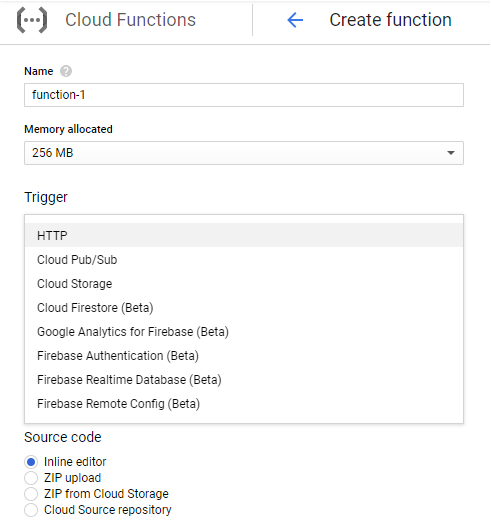
\includegraphics[width=12.5cm]{figuras/google-cloud-functions/triggers.png}
	\legend{Fonte: cloud.google.com/functions/}
	\label{fig:google-cloud-functions-triggers}
\end{figure}


\bigskip
Ou seja, apesar da versatilidade e facilidade de usar Google Cloud Functions, ela vem associada a muitas restrições de entrada e saída e também customizações de segurança.

\subsubsection{Linguagens}

Para os procedimentos e funções rodando no Cloud functions existe uma lista de possíveis linguagens de programação disponíveis, dentre essas linguagens temos Node.js, Python e Go.
Para o Node.js estão disponiveis as versões \textbf{Node.js 6} (deprecada), \textbf{Node.js 8}, \textbf{Node.js 10}, Para Python somente a versão \textbf{Python 3.7.1} e para Go somente \textbf{Go 1.11.65}.

\subsubsection{Escalabilidade}

TODO CONTINUE FROM HERE: https://cloud.google.com/functions/docs/concepts/exec

\subsubsection{Flexibilidade}

TODO

\subsection{Arquitetura}

TODO
\begin{figure}[ht]
	\centering
	\caption{Diagrama de funcionamento}
	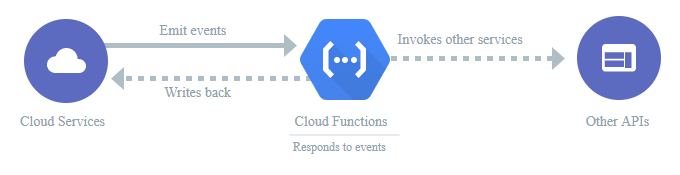
\includegraphics[width=12.5cm]{figuras/google-cloud-functions/workflow.png}
	\legend{Fonte: console.cloud.google.com}
	\label{fig:google-cloud-functions-workflow}
\end{figure}

\subsubsection{Protocolos de rede}

TODO

\subsubsection{Tolerância à falhas}

TODO

\subsection{Licença}

TODO

\subsection{Preço}

TODO

\subsection{Comparação}

TODO


\section{AWS Lambda}

O AWS Lambda é um serviço de computação em nuvem que segue o modelo de \textit{Serveless Computing}.
Ele permite que usuários façam implatação de serviços sem a necessidade de provisionamento ou gerenciamento da infraestrutura que os executarão.
De acordo com as afirmações feitas pela provedora do serviço:
o AWS Lambda executa o código do seu serviço em uma infraestrutura de computação de alta disponibilidade sem a necessidade da administração dos recursos computacionais, inclusive manutenção de servidor e sistema operacional, provisionamento de capacidade e escalabilidade automática, monitoramento do código e registro em log.


\subsection{Implantação}

TODO

\subsection{Escalabilidade}

TODO

\subsection{Flexibilidade}

TODO

\subsubsection{Linguagens}

TODO

\subsubsection{Entrada e saída}

TODO

\subsection{Arquitetura}

TODO

\subsubsection{Protocolos de rede}

TODO

\subsubsection{Tolerância à falhas}

TODO

\subsection{Licença}

TODO

\subsection{Preço}

TODO

\subsection{Propósito}

TODO

\subsection{Comparação}

TODO


\section{Apache Kafka}

TODO

\subsection{Implantação}

TODO

\subsection{Escalabilidade}

TODO

\subsection{Flexibilidade}

TODO

\subsubsection{Linguagens}

TODO

\subsubsection{Entrada e saída}

TODO

\subsection{Arquitetura}

TODO

\subsubsection{Protocolos de rede}

TODO

\subsubsection{Tolerância à falhas}

TODO

\subsection{Licença}

TODO

\subsection{Preço}

TODO

\subsection{Propósito}

TODO

\subsection{Comparação}

TODO


\section{Apache Storm}

TODO

\subsection{Implantação}

TODO

\subsection{Escalabilidade}

TODO

\subsection{Flexibilidade}

TODO

\subsubsection{Linguagens}

TODO

\subsubsection{Entrada e saída}

TODO

\subsection{Arquitetura}

TODO

\subsubsection{Protocolos de rede}

TODO

\subsubsection{Tolerância à falhas}

TODO

\subsection{Licença}

TODO

\subsection{Preço}

TODO

\subsection{Propósito}

TODO

\subsection{Comparação}

TODO


\chapter{CAPÍTULO 3}
\section{Exemplo de Tabelas, Quadros e Figuras}

{\centering\bfseries\color{red}
Exemplo de Tabela
\par}

\begin{table}[ht]
\centering
\caption{Preços de alimentos em dólares de 1900-1952 a
1995-1997}
\begin{supertabular}{m{3.6cm}m{3.7cm}m{3.6cm}m{3.0cm}}
\hline
\multicolumn{1}{m{3.636cm}|}{\centering{ ALIMENTO}} &
\multicolumn{1}{m{3.741cm}|}{\centering{ 1950-1952}} &
\multicolumn{1}{m{3.635cm}|}{\centering{ 1995-1977}} &
\centering\arraybslash{ VARIAÇÃO PERCENTUAL}\\\hline
\centering{ Trigo} &
\centering{ 427,6} &
\centering{ 159,3} &
\centering\arraybslash{ {}-62,7}\\
\centering{ Arroz} &
\centering{ 789,7} &
\centering{ 282,3} &
\centering\arraybslash{ {}-64,2}\\
\centering{ Sorgo} &
\centering{ 328,7} &
\centering{ 110,9} &
\centering\arraybslash{ {}-66,2}\\
\centering{ Milho} &
\centering{ 372,0} &
\centering{ 119,1} &
\centering\arraybslash{ {}-68,0}\\\hline
\end{supertabular}
    \legend{Fonte: Sen (2000, p. 240). }
    \label{tab:alimentos}
\end{table}

\bigskip

{\centering\bfseries\color{red}
Exemplo de Quadro
\par}

\begin{quadro}[htb]
\centering
\caption{Comparativo de competitividade}
\begin{supertabular}{|m{2.5cm}|m{2.5cm}|m{6.0cm}|m{3.0cm}|}
\hline
{ EMPRESA } &
{ PRINCIPAL MATÉRIA-PRIMA } &
{ ALTERNATIVAS DE SUPRIMENTOS PARA A PRINCIPAL MATÉRIA-PRIMA } &
{ FLEXIBILIDADE }\\\hline
{ Copesul } &
{ Nafta } &
{ Disponibilidade de produto na Argentina} &
{ 45\% condensado e GLP }\\\hline
{ Copene } &
{ Nafta } &
{ Alternativas Venezuela e Argélia } &
{ Inexistente }\\\hline
{ PQU } &
{ Nafta } &
{ Único fornecedor } &
{ Inexistente }\\\hline
{ Rio Polímeros } &
{ Etano } &
{ Único fornecedor } &
{ Inexistente }\\\hline
{ Baía Blanca } &
{ Etano } &
{ Projeto Mega / Única opção } &
{ Inexistente }\\\hline
\end{supertabular}
    \legend{Fonte: Freire e Jardim (2000, p. 78)}
    \label{quad:quadro1}
\end{quadro}

\bigskip
\clearpage

{\centering\bfseries\color{red}
Exemplo de Gráfico
\par}
\begin{figure}[ht]
    \centering
    \caption{Acesso à internet 1999 – 2002}
    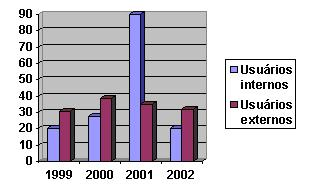
\includegraphics[width=12.5cm,height=7.2cm]{ModeloMonografiaDCCUFRJ-img002.png} 
    \legend{Fonte: Silva, Camargo Pires (2004, p. 45)}
    \label{fig:internet}
\end{figure}

\clearpage
\section{Exemplos de Citações}
{\centering\bfseries\color{red}
Exemplos de Citações
\par}

{\centering\bfseries\color{red}
Citação direta:
\par}

\bigskip

Citações diretas de até 3 linhas, devem iniciar e terminar por aspas duplas.\\

Se o texto original já contiver aspas duplas, substituí-las por aspas simples. A indicação da fonte da citação pode
estar inserida no texto ou após a citação.\\

\bigskip

{\color{red}
Exemplo:}

\bigskip

Segundo Castro (2001, p. 23): {\textquotedbl}Os deveres da conduta do anestesiologista constituem predicados importantes
quando se quer avaliar a qualidade do procedimento.{\textquotedbl}\\

\bigskip

{\color{red}
ou}

\bigskip

{
{\textquotedbl}A expressão 'furiosa' dessa estátua de que fala Rebelais, corresponde também à realidade.{\textquotedbl}
(BAKHTIN, 1987, p. 89).}

\bigskip

{\centering\bfseries\color{red}
Citação Direta com mais de três linhas:
\par}

\bigskip

As citações diretas, no texto, com mais de três linhas, devem ser
destacadas com recuo de 4 cm da margem esquerda, com letra menor que a do texto utilizado e sem as aspas. A indicação da fonte da citação pode estar inserida no texto ou após a citação. \\ 

\bigskip

{\color{red}
Exemplo:}
\bigskip
Sobre mercado financeiro, Fortuna (1996, p. 15) considera:\\
\bigskip

\begin{citacao}
O mercado financeiro permite que um agente econômico qualquer, sem perspectivas de aplicação, em algum empreendimento
próprio, da poupança que é capaz de gerar, seja colocado em contato com outro, cujas perspectivas de investimento
superam as respectivas disponibilidades de poupança.\\
\end{citacao}

\bigskip
A seguir uma citação em inglês:\\

\begin{citacao}[english]
This text is an example in English language in italic with correct hyphenation. This text is an example in English language in italic with correct hyphenation. This text is an example in English language in italic with correct hyphenation.
\end{citacao}
\bigskip

\clearpage{\centering\bfseries\color{red}
Citação Indireta:
\par}

\bigskip

Não se utilizam aspas para esse tipo de citação, nem a(s) página(s) de onde foi extraída a ideia.\\

\bigskip

{\color{red}
Exemplo:}

\bigskip

A bíblia começou a ser escrita no ano 1.000 a.C. e foi finalizada em 100 d.C., com a morte do último apóstolo, São João, levando aproximadamente 1.150 anos para ser concluída \cite{book:GHELLER}.\\


\bigskip

{\centering\bfseries\color{red}
Citação de Citação:
\par}

\bigskip

A indicação da fonte é feita pelo sobrenome do autor da obra citada (não consultada), ano, seguido da expressão latina apud. Após, indica-se o sobrenome do autor da obra consultada, seguido do ano de publicação, precedido por vírgula. Quando for citação direta incluir a(s) página(s) após a data de publicação, precedida de vírgula.\\

\bigskip

{\sffamily
\textrm{\textcolor{red}{Exemplo no texto}}\textrm{:}}

\bigskip

{\sffamily
\textrm{citado por }}

\bigskip

{\sffamily
\textrm{Segundo Marques e Ribeiro}\footnote{\ MARQUES, Alberto; RIBEIRO, \textbf{Angela. As fazendas agrícolas}. São
Paulo: Ática, 2000. 350 p.}\textrm{ (2000 }\textrm{\textcolor{black}{apud }}\textrm{OLIVEIRA, 2001), \apudonline {art:PRADO}{book:AMADO} o Serviço de
Atenção Médico-Sanitário da Suécia tem uma tradição de mais de cem anos. }}

\bigskip

{\color{red}
ou}

{\sffamily
\textrm{\textcolor{red}{Em nota de rodapé}}\textrm{:}}

\bigskip

{\centering\bfseries\color{red}
Indicação da Citação:
\par}

\bigskip

{\sffamily
\textrm{Se a indicação da fonte da citação estiver incluída na frase, a mesma deve aparecer apenas com a inicial
maiúscula seguida de parênteses, com a data de publicação do }\textrm{documento. Quando for citação direta incluir a(s)
página(s) após a data de publicação, precedida de vírgula.}}

\bigskip

{\color{red}
Exemplo com autor pessoal:}

\bigskip

Segundo Fonseca(2004, p. 36): {\textquotedbl}Se não houver mecanismos jurídicos que assegurem a proteção dos direitos
humanos, esse valor não será concretizado pelo Poder Público.{\textquotedbl}\\

\bigskip

{\sffamily
\textrm{\textcolor{red}{Exemplo com dois autores: }}}

\bigskip

Tonetto e Reck (2001, p. 134) destacam: {\textquotedbl}Este autoconhecimento pressupõe conhecer seus limites
[...]{\textquotedbl} \\

\bigskip

{\color{red}
Exemplo com mais de três autores:}

\bigskip

Neste contexto, Couto e outros (2004, p. 52) destacam que: {\textquotedbl}No capitalismo não é a simples ausência do
patrão que promove a superação do despotismo da divisão laboral.{\textquotedbl}\\

\bigskip

{\sffamily
\textrm{\textcolor{red}{Exemplo com autor institucional: }}}

\bigskip

De acordo com a Pontifícia Universidade Católica do Rio Grande do Sul (2001, p. 24): {\textquotedbl}[...] no horizonte 2001/2010, o esforço estratégico da PUCRS será centrado em sete áreas estratégicas [...]{\textquotedbl}\\

\bigskip

{\color{red}
Exemplo sem autor(es), com a entrada pelo título:}

\bigskip

Segundo o Guia de clareamento dental (1996, p. 8): {\textquotedbl}A causa mais comum do escurecimento dental é o tratamento endodôntico realizado de modo inadequado e sem os cuidados técnicos.{\textquotedbl}\\

\bigskip

{\color{red}
Exemplo sem autor(es), com a entrada pelo título que inicia por artigo:}

\bigskip

O movimento social, com o intuito de realizar uma transformação social, é uma das tarefas mais importantes da atualidade
(O COOPERATIVISMO..., 2002).\\

\bigskip

As citações a seguir foram colocadas para que as referências aparecessem na bibliografia. Como exemplo temos os livro de Jorge Amado \cite{book:AMADO}  \cite{book:AMADO2}, e este autor que desconheço \cite{book:OHANSSON}, além de \cite{book:ENGEL} e um artigo \cite{art:PRADO}. Notem que é gerado um link hipertexto no documento em PDF.


\chapter{Equações e Código}
\label{chp:capitulo4}

\section{Equações}
\label{sec:equacoes}
Referência: \url{http://en.wikibooks.org/wiki/LaTeX/Mathematics}

Também: \url{http://en.wikibooks.org/wiki/LaTeX/Advanced_Mathematics}

\begin{equation}
  (x + y)^2 = x^2 + 2xy + y^2
  \label{eq:equacao1}
\end{equation}

\section{Códigos}
\label{sec:codigos}
Reference: \url{http://en.wikibooks.org/wiki/LaTeX/Source_Code_Listings}

%\includecode[Linguagem]{Caption}{Label}{Arquivo}
\includecode[C]{Exemplo em Linguagem C} {alg:codigo1}{codigos/codigo.c}

%\includecode[Linguagem]{Caption}{Label}{Arquivo}
\includecode[Java]{Exemplo em Linguagem Java} {alg:codigo2}{codigos/codigo.java}

\section{Referências}
\label{sec:referencias}

A seguir como referenciar da maneira correta capítulos, seções, tabelas, etc. no texto corretamente.\\

\begin{itemize}
  \item Capítulo \ref{chp:capitulo4}
  \item Seção \ref{sec:codigos}
  \item Seção \ref{sec:referencias}
  \item Tabela \ref{tab:alimentos}
  \item Quadro \ref{quad:quadro1}
  \item Figura \ref{fig:internet}
  \item Equação \ref{eq:equacao1}
  \item Código \ref{alg:codigo1}
\end{itemize}

Para produzir um glossário em \Gls{latex} utilize o comando \emph{$\backslash$gls\{termo\}} para incluir a referência a um termo do glossário no texto. Um link de hipertexto será criado automaticamente para o termo no glossário como em \gls{maths}. 

As \glspl{formula} são processadas adequadamente e facilmente uma vez que o usuário se acostuma com os comandos. 
 
Dado um conjunto de números, há métodos elementares para calcular o seu \acrlong{mdc}, que é abreviado \acrshort{mdc}. Este processo é similar ao utilizado para o  \acrfull{mmc}.

Veja o arquivo glossario.tex em anexo para alguns exemplos simples.


\chapter{CONCLUSÃO}

Onde se expõe o fechamento das ideias do estudo, são apresentados os resultados da pesquisa, e partindo da análise destes resultados, tiram-se as conclusões e se for necessário, as sugestões relativas ao estudo. \\

Observação: É opcional a apresentação dos desdobramentos relativos à importância, síntese, projeção, repercussão, encaminhamento e outros.

\postextual
%%%%%%%%%%%%%%%%%%%%%%%%%%%%%%%%%%%%%%%%%%%%%%%%%%%%
% R E F E R Ê N C I A S  (OBRIGATÓRIO)
%%%%%%%%%%%%%%%%%%%%%%%%%%%%%%%%%%%%%%%%%%%%%%%%%%%%

\bibliography{elementos-postextuais/referencias.bib}

%%%%%%%%%%%%%%%%%%%%%%%%%%%%%%%%%%%%%%%%%%%%%%%%%%%%
% G L O S S A R I O (opcional)
%%%%%%%%%%%%%%%%%%%%%%%%%%%%%%%%%%%%%%%%%%%%%%%%%%%%
\clearpage
\addcontentsline{toc}{chapter}{GLOSSÁRIO} %\glossaryname
\printglossary

%%%%%%%%%%%%%%%%%%%%%%%%%%%%%%%%%%%%%%%%%%%%%%%%%%%%%%%%%
% A P Ê N D I C E S  (Opcional) 
%%%%%%%%%%%%%%%%%%%%%%%%%%%%%%%%%%%%%%%%%%%%%%%%%%%%%%%%%
%\textrm{\textcolor{red}{Apêndice(s) (Este item é elaborado 
% pelo próprio autor do trabalho e serve para  complementar
% a sua argumentação.  É um elemento \textbf{opcional)}.}}
%%%%%%%%%%%%%%%%%%%%%%%%%%%%%%%%%%%%%%%%%%%%%%%%%%%%%%%%

\clearpage
\begin{apendicesenv}

\begin{vplace}
{\centering
\ABNTEXchapterfont{\textrm{APÊNDICES}}
\par}
\end{vplace}
\newpage
{\let\clearpage\relax \chapter{\textnormal{Análise dos
	  relatórios mensais de uso do serviço de renovação de empréstimos.}}}

Lorem ipsum dolor sit amet, consectetur adipiscing elit. Donec lacus nisl,
ultricies vitae semper eu, scelerisque nec enim. Curabitur posuere tortor orci,
at porta leo laoreet et. Quisque ut congue dolor. Maecenas vel sagittis diam.
Praesent fermentum eleifend mi, sit amet vehicula leo pellentesque quis.
Curabitur mattis luctus pulvinar. Proin auctor est nec nulla pellentesque
commodo. Donec nec justo eu magna aliquet eleifend. Curabitur tristique tortor
id sem dignissim, a iaculis metus interdum. Phasellus bibendum velit sit amet
interdum semper. Nam vestibulum dui quis nisi consectetur, id vehicula dolor
faucibus.\\
\newpage
{\let\clearpage\relax \chapter{\textnormal{Análise dos
	  relatórios mensais de uso do serviço de empréstimo domiciliar.}}}

Lorem ipsum dolor sit amet, consectetur adipiscing elit. Donec lacus nisl, ultricies vitae semper eu, scelerisque nec enim. Curabitur posuere tortor orci, at porta leo laoreet et. Quisque ut congue dolor. Maecenas vel sagittis diam. Praesent fermentum eleifend mi, sit amet vehicula leo pellentesque quis. Curabitur mattis luctus pulvinar. Proin auctor est nec nulla pellentesque commodo. Donec nec justo eu magna aliquet eleifend. Curabitur tristique tortor id sem dignissim, a iaculis metus interdum. Phasellus bibendum velit sit amet interdum semper. Nam vestibulum dui quis nisi consectetur, id vehicula dolor faucibus.\\
\end{apendicesenv}

%%%%%%%%%%%%%%%%%%%%%%%%%%%%%%%%%%%%%%%%%%%%%%%%%%%%%%%%%
% A N E X O S   (Opcional) 
%%%%%%%%%%%%%%%%%%%%%%%%%%%%%%%%%%%%%%%%%%%%%%%%%%%%%%%%%
% \textrm{\textcolor{red}{Anexos (Este item é constituído por 
% documentos complementares ao texto do trabalho e que não são 
% elaborados pelo autor do mesmo, servem para fundamentação, 
% comprovação e ilustração. É um elemento \textbf{opcional}).}}
%%%%%%%%%%%%%%%%%%%%%%%%%%%%%%%%%%%%%%%%%%%%%%%%%%%%%%%%%

\clearpage
\begin{anexosenv}

\begin{vplace}
{\centering
\ABNTEXchapterfont{ANEXOS}
\par}
\end{vplace}
\newpage
{\let\clearpage\relax \chapter{\textnormal{Demonstrativo de
	  frequência diária ago./set. 2001}}}

Lorem ipsum dolor sit amet, consectetur adipiscing elit. Donec lacus nisl, ultricies vitae semper eu, scelerisque nec enim. Curabitur posuere tortor orci, at porta leo laoreet et. Quisque ut congue dolor. Maecenas vel sagittis diam. Praesent fermentum eleifend mi, sit amet vehicula leo pellentesque quis. Curabitur mattis luctus pulvinar. Proin auctor est nec nulla pellentesque commodo. Donec nec justo eu magna aliquet eleifend. Curabitur tristique tortor id sem dignissim, a iaculis metus interdum. Phasellus bibendum velit sit amet interdum semper. Nam vestibulum dui quis nisi consectetur, id vehicula dolor faucibus.\\
\newpage
{\let\clearpage\relax \chapter{\textnormal{Demonstrativo de frequência diária jan./dez. 2002}}}

Lorem ipsum dolor sit amet, consectetur adipiscing elit. Donec lacus nisl, ultricies vitae semper eu, scelerisque nec enim. Curabitur posuere tortor orci, at porta leo laoreet et. Quisque ut congue dolor. Maecenas vel sagittis diam. Praesent fermentum eleifend mi, sit amet vehicula leo pellentesque quis. Curabitur mattis luctus pulvinar. Proin auctor est nec nulla pellentesque commodo. Donec nec justo eu magna aliquet eleifend. Curabitur tristique tortor id sem dignissim, a iaculis metus interdum. Phasellus bibendum velit sit amet interdum semper. Nam vestibulum dui quis nisi consectetur, id vehicula dolor faucibus. \\

\end{anexosenv}

%%%%%%%%%%%%%%%%%%%%%%%%%%%%%%%%%%%%%%%%%%%%%%%%%%%%%%%%%
% F I M   D O  D O C U M E N T O
%%%%%%%%%%%%%%%%%%%%%%%%%%%%%%%%%%%%%%%%%%%%%%%%%%%%%%%%%
\end{document}
